\documentclass[border=10pt]{standalone}

\usepackage{tikz}
\usepackage{tikzsymbols}
\usetikzlibrary{calc,patterns,shapes.geometric}

\def\centerarc[#1](#2)(#3:#4:#5){\draw[#1] ($(#2)+({#5*cos(#3)},{#5*sin(#3)})$) arc (#3:#4:#5);}

\begin{document}
	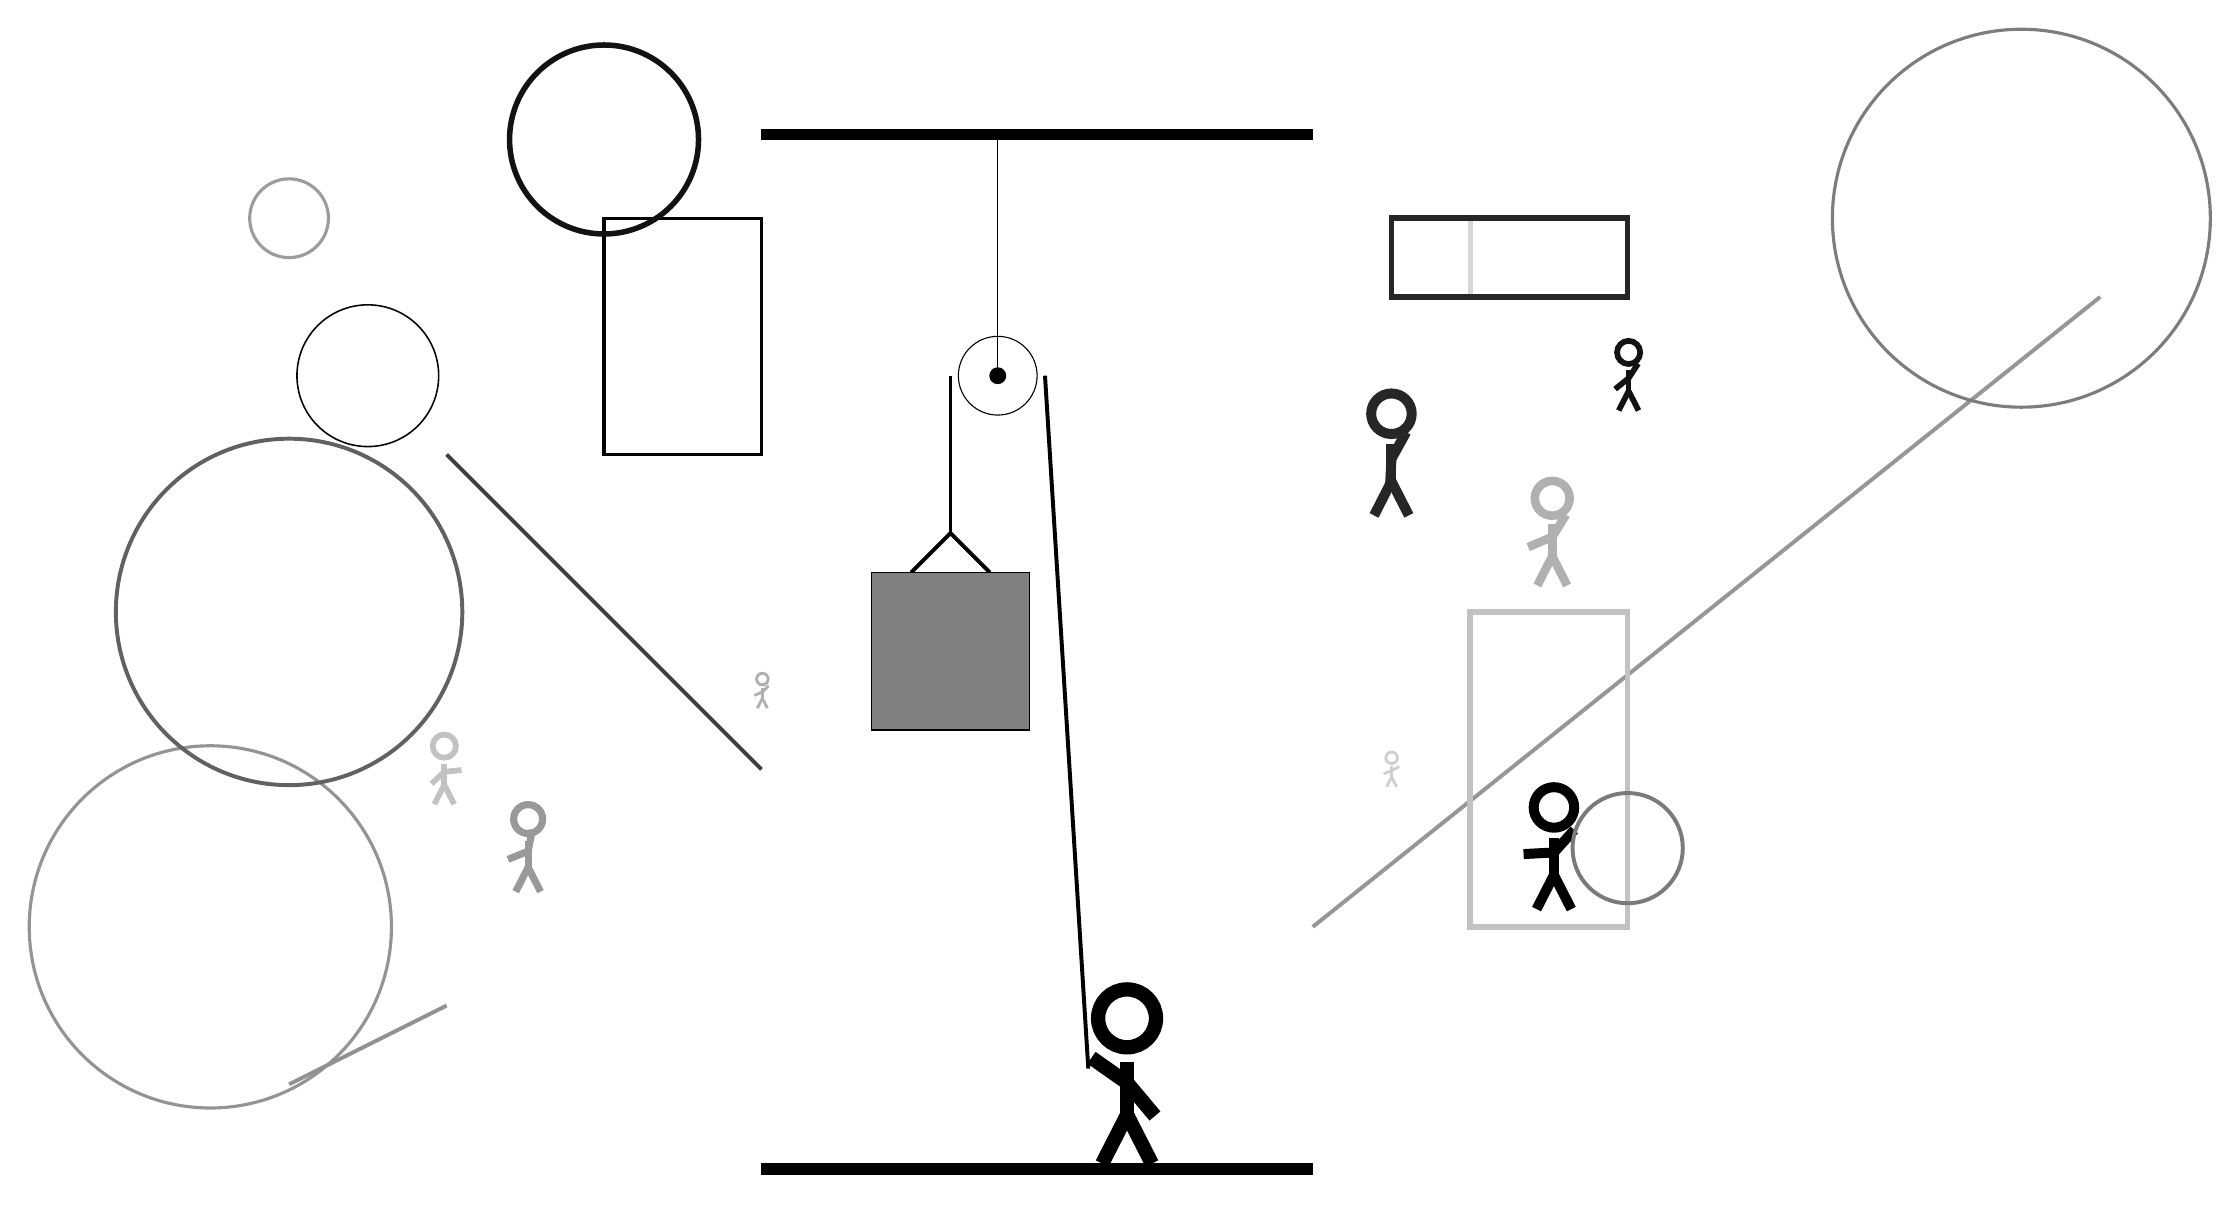
\begin{tikzpicture}
		%%%%% START %%%%%
		
		\draw[fill=black] (-2, 10) rectangle (5, 10.125);
		
		\draw (1, 7) circle (0.5);
		\draw[fill=black] (1, 7) circle (0.1);
		\draw (1, 10) -- (1, 7);
		
		\draw[line width=0.5mm] (-0.1, 4.5) -- (0.4, 5.0) -- (0.9, 4.5);
		\draw[fill=black!50] (-0.6, 4.5) rectangle (1.4, 2.5);
		
		\draw[line width=0.5mm] (0.4, 7) -- (0.4, 5.0);
		\centerarc[line width=0.5mm](1, 7)(0:180:0.6);
		\draw[line width=0.5mm](1.6, 7) -- (2.15, -1.8);
		
		\node at (2.6, -1.9) {\Strichmaxerl[10][-35][-50]};
		
		\node[line width=0.7mm, color=black!93] at (9, 7) {\Strichmaxerl[4][39][57]};
		
		\draw[line width=0.5mm, color=black!75](-6, 6) -- (-2, 2);
		\node[line width=0.5mm, color=black!40] at (-5, 1) {\Strichmaxerl[5][22][79]};
		\draw [line width=0.4mm, color=black!39](-8, 9) circle (0.5);
		\node[line width=0.5mm, color=black!100] at (8, 1) {\Strichmaxerl[7][3][48]};
		\draw[line width=0.5mm, color=black!41](5, 0) -- (15, 8);
		\draw [line width=0.4mm, color=black!42](-9, 0) circle (2.3);
		\node[line width=0.3mm, color=black!31] at (8, 5) {\Strichmaxerl[6][23][58]};
		\draw[line width=0.6mm, color=black!16] (7, 8) rectangle (7, 9);
		\draw [line width=0.5mm, color=black!62](-8, 4) circle (2.2);
		\draw[line width=0.4mm, color=black!99] (-4, 6) rectangle (-2, 9);
		\node[line width=0.7mm, color=black!24] at (-6, 2) {\Strichmaxerl[4][43][6]};
		\draw [line width=0.4mm, color=black!51](14, 9) circle (2.4);
		
		\node[line width=0.3mm, color=black!31] at (-2, 3) {\Strichmaxerl[2][24][44]};
		\draw[line width=0.7mm, color=black!85] (6, 8) rectangle (9, 9);
		\draw[line width=0.7mm, color=black!24] (7, 4) rectangle (9, 0);
		
		\node[line width=0.2mm, color=black!19] at (6, 2) {\Strichmaxerl[2][22][28]};
		\node[line width=0.4mm, color=black!85] at (6, 6) {\Strichmaxerl[7][87][61]};
		\draw [line width=0.2mm, color=black!98](-7, 7) circle (0.9);
		
		\draw [line width=0.5mm, color=black!52](9, 1) circle (0.7);
		\draw [line width=0.7mm, color=black!93](-4, 10) circle (1.2);
		\draw[line width=0.5mm, color=black!43](-6, -1) -- (-8, -2);
		
		\draw[fill=black] (-2, -3) rectangle (5, -3.15);
		
		%%%%% END %%%%%
	\end{tikzpicture}
\end{document}